\documentclass[conference]{IEEEtran}
\def\BibTeX{{\rm B\kern-.05em{\sc i\kern-.025em b}\kern-.08em
    T\kern-.1667em\lower.7ex\hbox{E}\kern-.125emX}}

\usepackage{./packages}

\title{Description of \textit{phipredictor}}

% \author{
% \IEEEauthorblockN{Guilherme Silva}
% \IEEEauthorblockA{
% Faculdade de Engenharia da Universidade do Porto\\
% Porto, Portugal\\
% up201603647@fe.up.pt}
% }
\addbibresource{references.bib}

\begin{document}

\maketitle

\section{Installation}

All code is encapsulated in a Python package called \verb|phipredictor| to 
install it simply clone it or download it and run the command \verb|python setup.py install|.
However, if further development is intended then the use the command
\verb|python setup.py develop| instead, so that the package automatically
updates when something changes in the source code. When developing it is also
recommended the use of a virtual environment, consult the
\href{https://docs.python.org/3/library/venv.html}{documentation}.

\section{Simulation}

The simulation is handled by the class \verb|PhaseSimulator| declared in the file
\verb|simulation.py|. The main interface with the class is made through the 
function \verb|simulate| which takes 3 arguments:

\begin{enumerate}
    \item \textit{mirror\_poses} - A matrix of size $(3,4)$ which describes
    the poses of the 4 mirrors;
    \item \textit{noise} - A boolean, when true adds Poisson noise to the
    end result, otherwise has no effect;
    \item \textit{symmetry} - A boolean, when false removes a square from the
    south mirror to remove any symmetries, otherwise has no effect.
\end{enumerate}

\section{Random Generation}

The generation of random samples is made using the class \verb|RandomSampler|
defined in the file \verb|random_sampler.py|. This file can be directly run 
to generate datasets. The command \verb|python random_sampler.py -h| shows 
all the options available, but the following is a brief overview.

\begin{itemize}
    \item \textit{output\_dir} - Required. The resulting dataset is going to be
    saved;
    \item \textit{-n N} - Number of examples to generate. Defaults to 500;
    \item \textit{-p} - If passed poisson noise is addeed to the generated samples;
    \item \textit{-s} - If passed symmetry is going to be eliminated
    in the generation.
\end{itemize}

The result of the generation consists a \verb|csv| file where each line
contains a file name and the corresponding mirror poses, and a folder containing
the files matching the file names in the csv, each of these contains the simulation
results.

\section{Model}

The model to be fitted to the simulated data is implemented in the file \verb|model.py|
using \verb|pytorch|.

\section{Training}

The training of the model can be done by executing the file \verb|train.py|, this script
has the following command line arguments:

\begin{enumerate}
    \item \textit{dataset} - Path to the root folder of the dataset;
    \item \textit{prefix} - Prefix of the folder name to which the results and 
    metrics are going to be saved to;
    \item \textit{-lr LR} - Learning rate of the optimizer, defaults to $10^{-5}$;
    \item \textit{-epochs EPOCHS} - Number of epochs to train for, defaults to 10;
    \item \textit{-batch BATCH} - Batch size to use at each training step, defaults to 4;
\end{enumerate}

As it stands the training as the following qualities:
\begin{itemize}
    \item 4 fold cross-validation is used;
    \item The loss function corresponds to the Mean Square Error;
    \item At the end of each epoch the average loss is calculated 
    for the entire validation fold;
    \item The optimizer corresponds to Stochastic Gradient Descent 
    (provided by \verb|pytorch|);
    \item The log function is applied to every example before it 
    used for training, this is necessary due to the high magnitude
    of the values in the samples.
\end{itemize}

\section{Results}

\begin{figure}[!t]
\centering
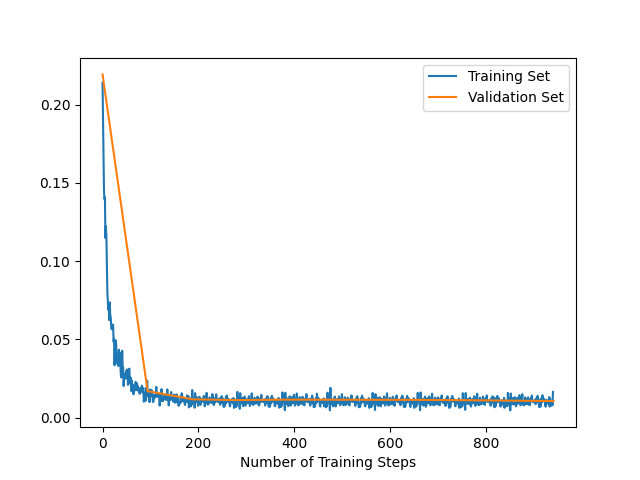
\includegraphics[width=2.8in]{images/results.png}
\caption{Training results with default values for learning rate and batch
size while using a dataset without the removal of symmetry}
\label{fig}
\end{figure}

As it can be clearly seen in Figure \ref{fig} the model already converged after the 
first epoch.

\section{Problems}


\end{document}